\documentclass{juliacon}
\usepackage{algorithm}
\usepackage{algpseudocode}
\usepackage{tikz}
\usetikzlibrary{patterns, arrows.meta}

\begin{document}

% **************GENERATED FILE, DO NOT EDIT**************

\title{A Fast, Stable Variant on Quicksort}

\author[1]{Lilith Hafner}
\author[1]{Kobina Thatcher}
\affil[1]{Independent Researcher}

\keywords{Julia, Performance, Sorting}



\maketitle

\begin{abstract}

% A brief summary of the paper, providing an overview of the research problem, methodology, main findings, and conclusions.

% We present a stable, out-of place variant of the Quicksort algorithm; prove its correctness, stability, and asymptotic performance characteristics; and empirically demonstrate that it outperforms conventional, unstable, Quicksort implementations on a variety of sorting tasks and architectures.

We present a Quicksort partitioning method that is stable and faster than existing partitioning methods on modern architectures at the cost of requiring auxiliary memory.

\end{abstract}

\section{Preliminaries}

See \cite{quicksort} for a description of Quicksort and \cite{lomuto} for generalizations to alternative partitioning schemes. This paper assumes familiarity with both. A video presentation of the proposed algorithm is available at \href{https://youtu.be/RIhCBTx5TYA}{youtu.be/RIhCBTx5TYA}

\section{Partitioning scheme}

The proposed partitioning scheme copies data from a source array to a destination array, partitioning it in the process. Compare each element of the source array with the pivot and fill the destination array from both ends, placing elements less than the pivot at the beginning and elements greater than the pivot at the end, as described in Algorithm \ref{alg:1}

\vspace{-5pt}

\begin{algorithm}[h]
\caption{Partitioning scheme}\label{alg:1}
\begin{algorithmic}[1]
  \Procedure{Partition}{$source$, $destination$, $pivot$}
    \State initialize $start \leftarrow$ pointer to first element of $destination$
    \State initialize $end \leftarrow$ pointer to last element of $destination$
    \For{each $element$ in $source$}
      \If{$element$ belongs before $pivot$}
        \State place $element$ at $start$
        \State increment $start$
      \Else
        \State place $element$ at $end$
        \State decrement $end$
      \EndIf
    \EndFor
    \State \Return $start$
  \EndProcedure
\end{algorithmic}
\end{algorithm}

% \begin{lstlisting}
% To partition from source to destitantion,
%     let start of free space = first index of destination
%     and let end of free space = last index of destination
%     for each element in source,
%         if the element is less than the pivot
%             put it at the start of free space
%             and increment free space.
%         Otherwise,
%             put it at the end of free space
%             and decrement end of free space.
% \end{lstlisting}

\vspace{-10pt}

\section{Stability}

Stability requires that elements which compare equivalently---neither is less than the other---appear in the output in the same order as in the input. We extend this to intermediary results and say that a block of memory is stable if every pair of equivalent elements in that block appears in the same order as in the input. We also define a notion of reverse-stability and say that a block of memory is reverse-stable if every pair of equivalent elements is in the opposite order as in the input.

After partitioning, elements less than the pivot appear at the start of the destination array in the same order they originally appeared and elements greater than the pivot appear at the end of destination array in reverse order. The reverse-stability of one sub-array is much more conducive to restoring stability than the complex mixing created by Hoare \cite{quicksort} and Lomuto \cite{lomuto} partitioning. We model stability in the Quicksort algorithm formed from the proposed partitioning scheme like so

\vspace{8pt}

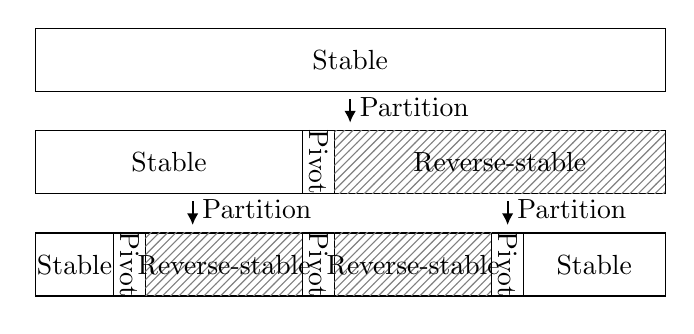
\begin{tikzpicture}
    % First rectangle
    \draw (0,0) rectangle (8,-.8);
    \node at (4,-0.4) {Stable};

    \draw[-{Latex[length=1.5mm, width=1.5mm]}, thick] (4,-0.9) -- (4,-1.2);
    \node at (4,-1.0) [right] {Partition};

    % Second rectangle
    \draw (0,-1.3) rectangle (8,-2.1);
    \node at (1.7,-1.7) {Stable};
    \draw (3.4,-1.3) -- (3.4,-2.1);
    \node[rotate=270] at (3.6,-1.7) {Pivot};
    \draw (3.8,-1.3) -- (3.8,-2.1);
    \fill[pattern=north east lines, pattern color=gray] (3.8,-1.3) rectangle (8,-2.1);
    \node at (5.9,-1.7) {Reverse-stable};

    \draw[-{Latex[length=1.5mm, width=1.5mm]}, thick] (2,-2.2) -- (2,-2.5);
    \node at (2,-2.3) [right] {Partition};

    \draw[-{Latex[length=1.5mm, width=1.5mm]}, thick] (6,-2.2) -- (6,-2.5);
    \node at (6,-2.3) [right] {Partition};

    % Third rectangle
    \draw (0,-2.6) rectangle (8,-3.4);
    \node at (0.5,-3.0) {Stable};
    \draw (1.0,-2.6) -- (1.0,-3.4);
    \node[rotate=270] at (1.2,-3.0) {Pivot};
    \draw (1.4,-2.6) -- (1.4,-3.4);
    \fill[pattern=north east lines, pattern color=gray] (1.4,-2.6) rectangle (3.4,-3.4);
    \node at (2.4,-3.0) {Reverse-stable};
    \draw (3.4,-2.6) -- (3.4,-3.4);
    \node[rotate=270] at (3.6,-3.0) {Pivot};
    \draw (3.8,-2.6) -- (3.8,-3.4);
    \fill[pattern=north east lines, pattern color=gray] (3.8,-2.6) rectangle (5.8,-3.4);
    \node at (4.8,-3.0) {Reverse-stable};
    \draw (5.8,-2.6) -- (5.8,-3.4);
    \node[rotate=270] at (6,-3.0) {Pivot};
    \draw (6.2,-2.6) -- (6.2,-3.4);
    \node at (7.1,-3.0) {Stable};
\end{tikzpicture}

\vspace{8pt}

Each partition splits the input into a stable sub-array and a reverse-stable sub-array where the first sub-array is of the same stability as the partition's input and the second sub-array is the opposite stability. Further, any pair of equivalent elements separated by a pivot always appear in the same order as they do in the input.

\begin{algorithm}[h]
\caption{Stable partitioning scheme}\label{alg:split}
\begin{algorithmic}[1]
  \Procedure{Partition}{$source$, $destination$, $pivot\_index$}
    \State initialize $pivot \leftarrow source[pivot\_index]$
    \State initialize $start \leftarrow$ pointer to first element of $destination$
    \State initialize $end \leftarrow$ pointer to  last element of $destination$
    \For{each $element$ in $source$ before $pivot\_index$}
      \If{$element \le pivot$}
        \State place $element$ at $start$
        \State increment $start$
      \Else
        \State place $element$ at $end$
        \State decrement $end$
      \EndIf
    \EndFor
    \For{each $element$ in $source$ after $pivot\_index$}
      \If{$element < pivot$}
        \State place $element$ at $start$
        \State increment $start$
      \Else
        \State place $element$ at $end$
        \State decrement $end$
      \EndIf
    \EndFor
    \State place $pivot$ at $start$ (which is now equal to $end$)
    \State \Return $start$
  \EndProcedure
\end{algorithmic}
\end{algorithm}

Elements less than and greater than the pivot are handled well by Algorithm \ref{alg:1}. However, elements equal to the pivot must be placed after the pivot iff they occur after the pivot in the input. This can be handled by a complex "belongs before" comparison which accounts for both position and value but it is more efficient to split the partitioning loop in two. First iterate over elements before the pivot, branching on whether they are less than or equivalent to the pivot element; and then iterate over elements after the pivot, branching on whether they are strictly less than the pivot. Concretely, this may be implemented as Algorithm \ref{alg:split}

% \vspace{20pt}

% \begin{lstlisting}[language=Julia]
% function partition!(destination, source, pivot_index)
%     pivot = source[pivot_index]
%     destination_start = firstindex(destination)
%     destination_end = lastindex(destination)
%     for element in @view source[begin:pivot_index-1]
%         if element <= pivot # Loose inequality
%             destination[destination_start] = element
%             destination_start += 1
%         else
%             destination[destination_end] = element
%             destination_end -= 1
%         end
%     end
%     for element in @view source[pivot_index+1:end]
%         if element < pivot # Strict inequality
%             destination[destination_start] = element
%             destination_start += 1
%         else
%             destination[destination_end] = element
%             destination_end -= 1
%         end
%     end
%     @assert destination_start == destination_end
%     destination[destination_start] = pivot
% end
% \end{lstlisting}

To stabilize the final result we use a stable sorting algorithm as the base case for stable base cases and a reverse-stable sorting algorithm for reverse-stable base cases. Reverse-stable sorting algorithms are not the focus of this paper and can easily be formed by reversing an input and then applying a stable sorting algorithm such as insertion sort.

\section{Empirical performance}

To measure the practical efficiency of this partitioning scheme we implement it and existing partitioning schemes in the Julia \cite{julia} programming language.

We benchmark simple Quicksort implementations using the Hoare, Lomuto, and proposed partitioning schemes, as well as algorithms from Julia's standard library. All benchmarked algorithms use Insertionsort as a base case for 20 or fewer elements. Only the proposed algorithms and Mergesort are stable.

Additionally, we benchmark an optimized implementation of Quicksort using the proposed partitioning scheme. These optimizations include manual stack---or nest, as Hoare calls it---management, stable median-of-three pivot selection, and a base case that integrates reversing and copying with insertion sort.

\vspace{8pt}

\scalebox{.5}{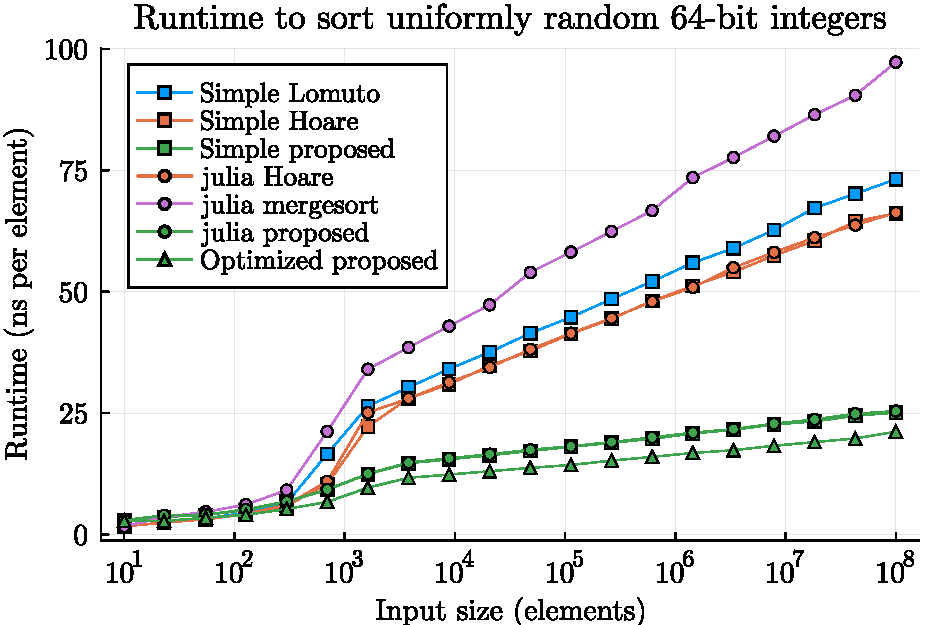
\includegraphics{runtime.pdf}}

\vspace{8pt}

As input size increases, the proposed partitioning scheme significantly outperforms existing systems, despite the additional memory usage and time taken to allocate scratch space. This improvement over prior art dwarfs additional improvements such as median of three partitioning, nest management, and some base-case optimization.

The relative performance of the discussed algorithms are similar for various bitwidth integers and floating point numbers, as well as records containing a key that does not occupy the entire record. However, there are cases with different trends. Notably, when the data are already sorted, reverse sorted, or all keys are identical. In these cases, Hoare partitioning reliably but marginally outperforms the proposed partitioning scheme.

\vspace{8pt}

\scalebox{.5}{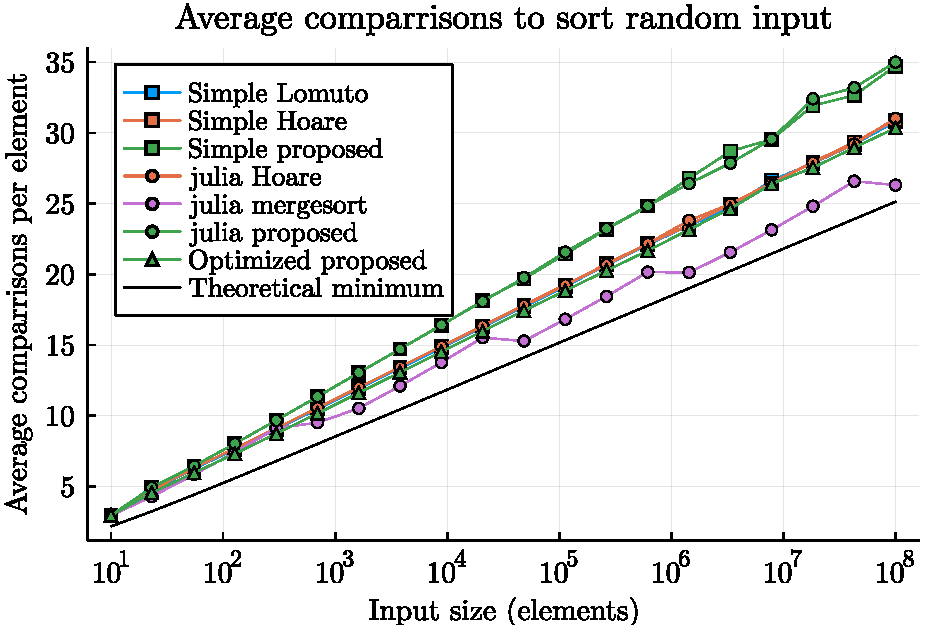
\includegraphics{comparrisons.pdf}}

\vspace{5pt}

Additionally, Mergesort performs fewer comparisons than any of the studied partitioning schemes. While Mergesort is significantly slower than the proposed partition scheme when comparisons are cheap, when comparisons are substantially more resource-intensive Mergesort will outperform all studied Quicksorts.

\subsection{Reproducibility}

The data were generated on a dedicated 2022 Apple M2 system with 8GB of memory and are qualitatively similar to results produced on a shared ProLiant DL325 Gen10 Plus v2. They can be reproduced on additional hardware by installing the Julia package hosted at \href{https://github.com/LilithHafner/QuickerSort.jl}{github.com/LilithHafner/QuickerSort.jl} and running \lstinline{QuickerSort.reproduce_figures()}.

\section{Deployment and reference implementations}

The proposed partitioning scheme is used in Julia's the default sorting algorithm due to superior performance over the prior Hoare partitioning method\cite{PR}. The implementations used for benchmarking are available at \href{https://github.com/LilithHafner/QuickerSort.jl}{github.com/LilithHafner/QuickerSort.jl}.

\section{Role in an in-place sorting algorithm}

All algorithms require $\Omega(1)$ auxiliary memory. This memory can be used as scratch space for the proposed partitioning scheme provided the length of inputs provided to that partitioning scheme is bounded. This enables the use of the proposed algorithm as a base case for stable, in-place, divide and conquer sorting algorithms such as paged mergesort \cite{pagedmergesort}

%For a more modest reduction in auxiliary memory usage, it is possible to perform the proposed Quicksort variant on the first and second half of a vector separately and then merge the results, with all operations using the same scratch space of size $n/2$.

% **************GENERATED FILE, DO NOT EDIT**************

\bibliographystyle{juliacon}
\bibliography{ref.bib}


\end{document}

% More discusssion of results
% - Cache size